\hypertarget{arrivuxe9e-au-pays-des-mille-oiseaux}{%
\section{Arrivée au pays des mille
oiseaux}\label{arrivuxe9e-au-pays-des-mille-oiseaux}}

\emph{Dimanche 22 juillet 2018}

Changement d'hémisphère, de saison, perte de plus de 20 degrés et de 4
heures d'ensoleillement par jour, shorts rangés, de l'anglais partout
autour de nous (mais avec un accent bizarre quand même) : pas de doute,
on est bien arrivés en Australie ! Et on a été accueillis royalement par
Svenja et Rémi, expatriés dans le pays du kangourou depuis de nombreuses
années, qui nous ont ouvert leurs portes à Sydney.

\begin{figure}
\centering
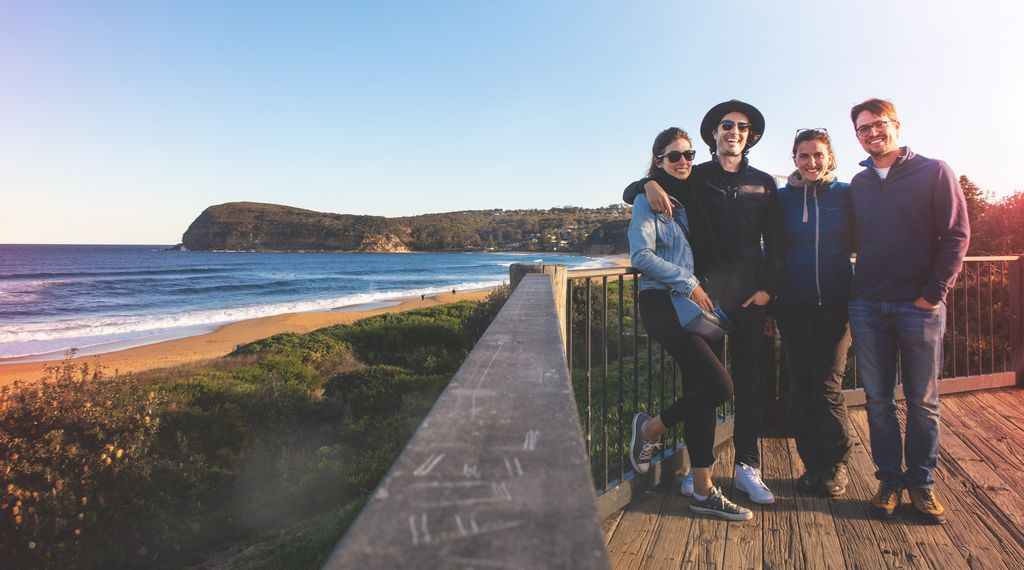
\includegraphics{images/20180724_australie.jpg}
\caption{Avec nos hôtes, excursion sur la Central Coast.}
\end{figure}

Et l'Australie fait déjà son petit effet sur nous : certes c'est
l'hiver, mais cela n'empêche pas les petits déjeuners sur la terrasse,
avec des perroquets aux couleurs vives qui viennent réclamer un bout de
pain, les balades sur la plage à observer les surfeurs, et même le
passage de quelques baleines à l'horizon...

On vous raconte ça très vite !

\begin{figure}
\centering
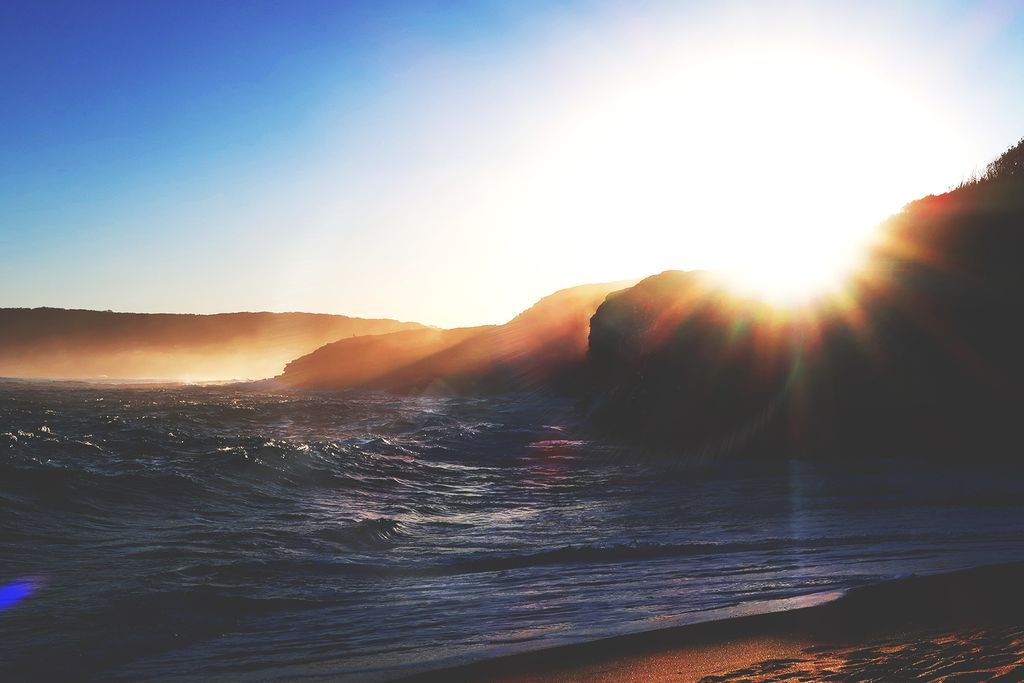
\includegraphics{images/20180724_plage.jpg}
\caption{Coucher de soleil sur Bouddi Beach.}
\end{figure}

\emph{Elida et Florian}
